% !TEX TS-program = lualatex

\documentclass[12pt]{scrartcl}
\usepackage[utf8]{inputenc}
\usepackage[spanish,mexico]{babel}
\usepackage{amsmath}
% \usepackage{amsfonts}
% \usepackage{amssymb}
\usepackage{amsthm}
\usepackage{caption}
\usepackage{subcaption}

\captionsetup{format=plain,labelfont=it}
\captionsetup{belowskip=-5pt}
\usepackage{setspace}
\onehalfspacing % doble espacio
% \doublespacing
\theoremstyle{definition}
\newtheorem{defi}{Definición}[section]
\DeclareMathOperator*{\argmax}{argmax}
\usepackage{multirow,array}
\usepackage{graphicx}
\RequirePackage[table]{xcolor} 
\definecolor{maroon}{cmyk}{0,0.87,0.68,0.32}
% \usepackage[dvipsnames]{xcolor}
\usepackage{multicol}
\usepackage{paracol}
\usepackage{vmargin}  % Administrar márgenes
\setpapersize{A4} % Definir tamaño del papel
\setmargins{2cm} % Margen izquierdo
{1cm} % Margen superior
{17cm} % Área de impresión horizontal
{24.42cm} % Area de impresión vertical
{15mm} % Encabezado
{5mm} % Espacio entre el encabezado y el texto
{10pt} % Pie de página
{3mm} % Espacio entre el pie de página y el texto
\usepackage{fancyhdr}
\usepackage{float}
\usepackage{hyperref}
\usepackage{istgame}
\usepackage{forest}
\usepackage{sgamex}
\usepackage[charter,cal=cmcal]{mathdesign}
\usepackage[T1]{fontenc}
% \usepackage{euler}
% \usepackage{eulervm}

% bold vector
\newcommand{\vect}[1]{\boldsymbol{#1}}    
\fancypagestyle{plain}{
	\fancyhead[r]{\textbf{Decisiones y Teoría de Juegos \\ Ingeniería Financiera \\ ITESO \\ \date{\today}}}
	\renewcommand{\headrulewidth}{0pt}
}
% Cajas y dibujos
\usepackage[most,breakable,skins]{tcolorbox}
\usepackage{tikz}

\usetikzlibrary{calc}
\newcommand*\circled[1]{\tikz[baseline=(char.base)]{
    \node[shape=circle, draw, inner sep=1pt, fill=gray!15,
        minimum height={.5cm}] (char) {\vphantom{WAH1g}#1};}} % \f@size*1.6 in height
\makeatother

\forestset{
     declare toks={elo}{}, % Edge Label Options
     anchors/.style={anchor=#1,child anchor=#1,parent anchor=#1},
     dot/.style={tikz+={\fill (.child anchor) circle[radius=#1];}},
     dot/.default=2pt,
     decision edge label/.style n args=3{
     edge label/.expanded={node[midway,auto=#1,anchor=#2,\forestoption{elo}]{\strut$\unexpanded{#3}$}}
     },
     decision/.style={if n=1
     {decision edge label={left}{east}{#1}}
     {decision edge label={right}{west}{#1}}
     },
     decision tree/.style={
     for tree={
     s sep=0.5em,l=8ex,
     if n children=0{anchors=north}{
     if n=1{anchors=south east,fill=raspberry!10}{anchors=south west,fill=raspberry!10}},
     math content
     },
     anchors=south, outer sep=2pt,
     dot=3pt,for descendants=dot,
    %  dot={fill=white},for descendants={dot={fill}},
     delay={for descendants={split option={content}{;}{content,decision}}},
     }
 }

 \usepackage{pgfplots} 
\pgfplotsset{compat=newest}
\pgfplotsset{plot coordinates/math parser=false}
\pgfplotsset{
    every non boxed x axis/.style={
        xtick align=center,
        enlarge x limits=true,
        x axis line style={line width=0.8pt, -latex}
},
    every boxed x axis/.style={}, enlargelimits=false
}
\pgfplotsset{
    every non boxed y axis/.style={
        ytick align=center,
        enlarge y limits=true,
        y axis line style={line width=0.8pt, -latex}
},
    every boxed y axis/.style={}, enlargelimits=false
}
\usetikzlibrary{
   arrows.meta,
  intersections,
}

\newtcolorbox{mybox}[2][]{%
	enhanced,
	breakable,
    frame hidden,
    overlay broken = {(frame.north west) rectangle (frame.south east);},
    colback=gray!9, 
	colbacktitle=raspberry!10!white,
	colback=blue!9!white,
	coltitle=blue!90!black,
	attach boxed title to top left={xshift=1cm,yshift=-\tcboxedtitleheight/2,yshifttext=-\tcboxedtitleheight/2},
	%attach boxed title to top center={yshift=-2mm},
	title={#2},
	%drop fuzzy shadow southeast,%=black!50!white,
	fonttitle=\bfseries\sffamily,
	#1
}
% summarybox

\newtcolorbox{summarybox}[2][]{
    enhanced,
	breakable,
    frame hidden,
    overlay broken = {
        % \draw[line width=1mm, red, rounded corners]
        (frame.north west) rectangle (frame.south east);},
    colback=gray!9, 
    colframe=white, 
    coltitle=black,
    fonttitle=\bfseries\sffamily,
    title={#2},
    #1}
% Definir una caja de ejemplos
\newtcolorbox{exbox}[2][]{
    enhanced,
	breakable,
    frame hidden,
    overlay broken = {
        (frame.north west) rectangle (frame.south east);},
    colbacktitle=gray!10,
    colback=bluerow!40,
    colframe=bluerow!40,
    coltitle=black,
    attach boxed title to top left={xshift=1cm,yshift=-\tcboxedtitleheight/2,yshifttext=-\tcboxedtitleheight/2},
    fonttitle=\bfseries\sffamily,
    title={#2},
    #1}

\newenvironment{myitemize}
{ \begin{itemize}
		\setlength{\itemsep}{0pt}
		\setlength{\parskip}{0pt}
		\setlength{\parsep}{0pt}     }
	{ \end{itemize}                  } 
	
\newenvironment{myenum}
{ \begin{enumerate}
		\setlength{\itemsep}{0pt}
		\setlength{\parskip}{0pt}
		\setlength{\parsep}{0pt}     }
	{ \end{enumerate}                  } 
	
\usepackage{fontawesome}
% Color definitions
\definecolor{raspberry}{rgb}{0.89, 0.04, 0.36}
\definecolor{yelltcol}{HTML}{FEE581}
% Tablas con line break automático
\usepackage{tabularx}
% Colores para tabla

\definecolor{bluerow}{HTML}{D5E5FF}
\definecolor{redrow}{HTML}{FFAAAA}
\definecolor{purplerow}{HTML}{FFAAEE}

\newcommand{\Cross}{\mathbin{\tikz [x=1.4ex,y=1.4ex,line width=.1ex] \draw (0,0) -- (1,1) (0,1) -- (1,0);}}%


% Definiciones de simbolos 
\newcommand\independent{\protect\mathpalette{\protect\independenT}{\perp}}
\def\independenT#1#2{\mathrel{\setbox0\hbox{$#1#2$}%
		\copy0\kern-\wd0\mkern4mu\box0}} 

\decimalpoint

\lhead{
	\begin{picture}(0,0)
	\put(0,0){
\includegraphics[scale=1.1]{logo_ITESO}}
	\end{picture}
}
\pagestyle{fancy}

\title{Notas de Unidad 1\\ \textbf{Preliminares}\\ \normalsize Decisiones y Teoría de Juegos}
\author{Emmanuel Alcalá}
\date{\today}

\begin{document}
\setlength{\parskip}{5mm}
\maketitle

\section{Revisión de matemáticas}
\subsection{Definiciones básicas}

\begin{description}

\item[Suma con notación $\Sigma$] - Suma de $i$ elementos hasta $n$, donde $i$ el índice de sumación

\begin{center}
    $\sum_{i=m}^n x_i=x_1 + x_2 + ... + x_n$
\end{center}

Donde $m$ es el límite inferior de la suma, y $n$ el límite superior de la suma. 

Ejemplo:

\begin{center}
    $x=\{1, 2, 3, 5 \}$ \\
    $\sum_{i=2}^{4} = 2 + 3 + 5 = 10$
\end{center}

\item[Conjuntos y subconjuntos] - Un conjunto es una colección de distintos objetos. $A$ es un subconjunto de $B$ si todo elemento de $A$ es también incluido en $B$, que se simboliza como $A \subset B$. \\
El conjunto vacío, denotado $\emptyset$, es el conjunto que no contiene nada.\\
Denotamos por $|S|$ a la cardinalidad (maomeno \textit{el número de sus elementos}) de $S$. Por ejemplo, $|\emptyset|=0$. \\
$x \in A$ es "$x$ es un miembro del conjunto $A$".

\item[Producto cartesiano.] $\Cross_{i=1}^n S_i = \prod_{i=1}^n S_i = S_1 \times S_2 \times ... \times S_n$.\\
Donde $S$ es un conjunto (\textit{set}). El producto cartesiano $S_1 \times S_2$ retorna un nuevo conjunto de todos los pares ordenados, con el primer elemento de $S_1$ y el segundo de $S_2$.\\
Ejemplo:\\
$A = \{1, 2\}$, $B = \{5, 6\}$. El producto $A\times B = \{(1, 5), (1, 6), (2, 5), (2, 6) \}$

	\item[Valor esperado] - (a.k.a.~\emph{media}, \emph{esperanza}, o \emph{promedio}) es una suma ponderada de los posibles resultados de nuestra variable aleatoria. Matemáticamente, si $x_1, x_2, x_3, \dots$ son todas distintos posibles valores que $X$ puede tomar, el valor esperado de $X$ es
	\begin{align*}
		E[X] &= \sum\limits_{i}x_i p(X=x_i), \text{ si $x$ es discreta}\\
		E[X] &= \int_\mathbb{R} xf(x)dx, \text{ si $x$ es continua}
	\end{align*}
	
	Por brevedad, podemos simplemente escribir $p(x_i)$ para el caso discreto. Para el caso continuo, $f(x)$ denota la función de densidad de probabilidad.
	
	Si tenemos $n$ datos, todos con la misma probabilidad de ser tomados por $X$, entonces la esperanza es simplemente la media aritmética:
	
	\begin{center}
		$E[X] = \frac{1}{n}\sum\limits_{i}x_i = \frac{x_1 + x_2 + \dots + x_n}{n}$
	\end{center}
	
	Con $p(x_1)=p(x_2)=...=p(x_n)=1/n$.

    \textbf{LOTUS: Law of the unconscious statistician} si $ g(x) $ es una transformación de no identidad de $ x $, $ E[g(X)] $ tiene el mismo significado:


    \[
        E[X] = \sum\limits_{i} g(x_i) p(x_i)
    \]

    Este teorema nos sirve para lo siguiente: si conocemos la probabilidad de $ x $ pero no la de $ g(x) $ aún podemos calcular el valor esperado de $ g(x) $. 
    
    Notar que si la transformación $ g(x) = x $ (identidad), $ E[g(X)] = E[X] $. 

	\item[Linealidad] - Para cualesquier variables aleatorias $X$ y $Y$, y constantes $a,b,c,$ 
	\[E(aX + bY + c) = aE[X] + bE[Y] + c \]
	
	\begin{minipage}{\linewidth}
		\centering
		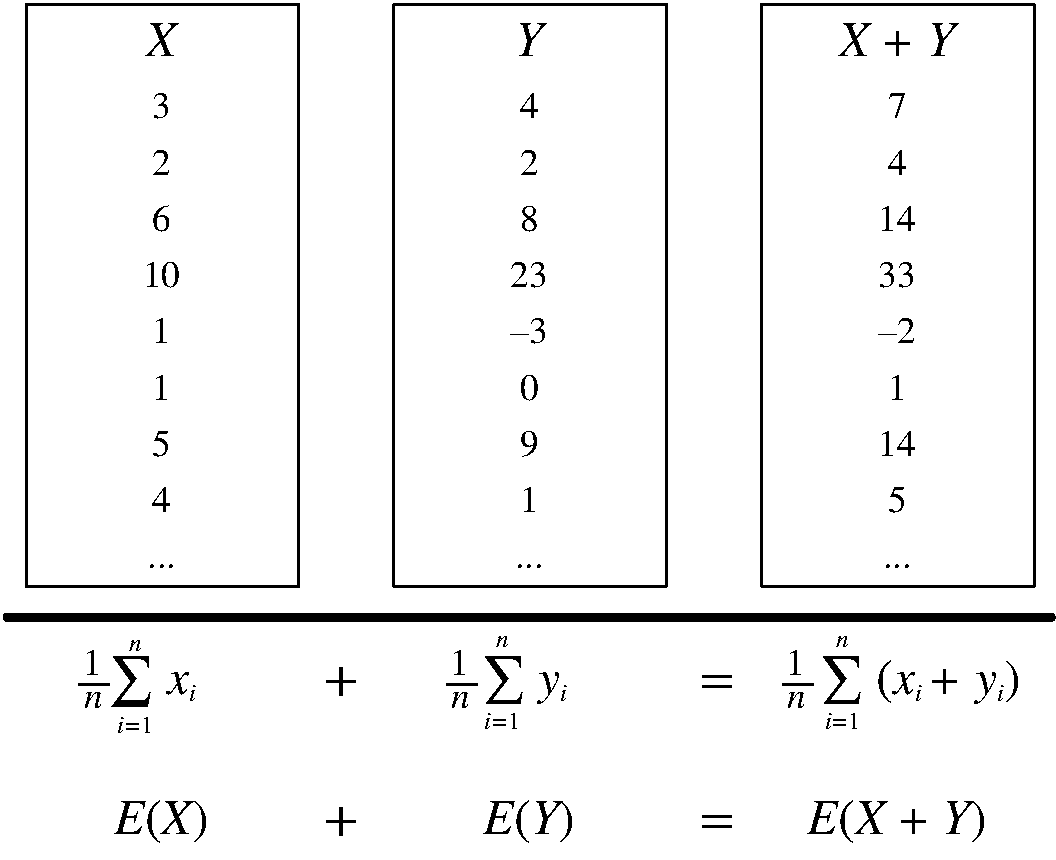
\includegraphics[width=3in]{figs/linearity.pdf}
	\end{minipage}
	
% 	{\textit{Ejercicio:} resolver el problema de la figura para los primeros 5 números de $X, Y$. Resolver cuando $a=2, b=0.5, c=10$.}
	
% 	\item[Algunas distrubuciones implican la misma media] - Si $X$ y $Y$ tienen la misma distribución, entonces $E(X)=E(Y)$ y, más generalmente, 
% 	$$E(g(X)) = E(g(Y))$$
	
	\item[Definición naïve de probabilidad] - {Si todos los resultados son igualmente posibles}, la probabilidad de un evento $A$ ocurriendo es:
	\[P_{\textrm{naïve}}(A) = \frac{\textnormal{veces que sale $A$}}{\textnormal{total de resultados (i.e., $A \cup A^c$})} = \frac{|A|}{|S|}\]
	
	Donde por $|\cdot|$ entendemos la \textit{cardinalidad}, o el número de elementos. 
	\item[Probabilidad] - Variables y espacios:
	
		\textbf{Variable aleatoria}: es una función que mapea los resultados de un experimento aleatorio al conjunto de los números reales (comúnmente). Se suele representar con letra mayúscula (e.g., $X$).

		\textbf{Espacio muestral}: el conjunto de todos los resultados posibles. Se suele representar con $\Omega$. De este conjunto la $X$ mapea a los reales: $X: \Omega \rightarrow \mathbb{R}$. Es decir, a cada elemento de $\Omega$ asigna un número real, $X(\omega)$.

		\textbf{Evento}: subconjunto de $\Omega$, usualmente representado por una vocal mayúscula, e.g., $A$. Si lanzamos una moneda dos veces, $\Omega = \{HH,HT,TT,TH\}$. El evento ``la primera moneda cae H'' es $A=\{HH,HT\}$. 

		\item[Axiomas de Kolmokorov] - La función $p(A)$ asigna un valor numérico a cada evento $A$. Se llama probabilidad de $A$ si satisface los siguientes axiomas:
		\begin{itemize}
			\item \textbf{Axioma 1:} $p(A) \geq 0$ para cada $A$. Es decir, $p(A)$ es positiva.
			\item \textbf{Axioma 2:} $p(\Omega) = 1$.
			\item \textbf{Axioma 3:} para los eventos $A_i,A_j..., i \neq j$ (es decir, si son disjuntos), 
			\[p\Bigg (\bigcup^\infty_{i=1} A_i \Bigg) = \sum_{i=1}^{\infty} p(A_i)\]
		\end{itemize}
	
	\item[El valor esperado condicional] es definido como la esperanzas, solo que condicionado a cualquier evento $A$.
	\begin{center}
		$\ E(X | A) = \sum\limits_{x}p(x|A)x$
	\end{center}
	
	\item[Función convexa] - Una función $f\colon \mathrm{I} \mapsto \mathbb{R}$ es convexa si para todo $x_1, x_2 \in \mathrm{I}, x_1 < x_2$, existe un $\lambda \in [0, 1]$ tal que 
	
	% \begin{center}
	%     $$
	% \end{center}
    \[
        f[\lambda x_1 + (1 - \lambda)x_2] \leq \lambda f(x_1) + (1-\lambda)f(x_2)\quad \forall x_1,x_2\in \mathrm{I}  \text{ y } \forall \lambda \in [0, 1]    
    \]
	\begin{summarybox}[colback=red!15]{Nota}
		$\forall \Longleftrightarrow \text{para todos; para cada uno}$. \\
		La combinación lineal $\lambda x_1 + (1 - \lambda)x_2$ es llamada \textit{combinación convexa}. Es equivalente a $y + \lambda(x_1-x_2)$.
	\end{summarybox}

    \begin{tikzpicture}
        \begin{axis}[width=5in,axis equal image,
            axis lines=middle,
            xmin=0,xmax=8,
            xlabel=$x$,ylabel=$y$,
            ymin=-0.25,ymax=4,
            xtick={\empty},ytick={\empty}, axis on top
        ]
        
        % 
        \addplot[thick,domain=0.25:7,red!90!black,name path = A]  {-x/3 + 2.75} coordinate[pos=0.4] (m) ;
        \draw[thick,blue, name path =B] (0.15,4) .. controls (1,1) and (4,0) .. (6,2) node[pos=0.95, color=black, right]  {$f(x)$} coordinate[pos=0.075] (a1)  coordinate[pos=0.95] (a2);
        \path [name intersections={of=A and B, by={a,b}}];
        
        % 
        \draw[densely dashed] (0,0) -| node[pos=0.5, color=black, label=below:$a$] {}(a1);
        \draw[densely dashed] (0,0) -| node[pos=0.5, color=black, label=below:$x_{1}$] {}(a);
        \draw[densely dashed, name path=D] (3,0) -|node[pos=0.5, color=black, label=below:$\lambda x_{1}+ (1-\lambda)x_{2}$] {} node[pos=1, fill,circle,inner sep=1pt] {}(m);
        \draw[densely dashed] (0,0) -|node[pos=0.5, color=black, label=below:$x_{2}$] {}(b);
        \draw[densely dashed] (0,0) -|node[pos=0.5, color=black, label=below:$b$] {}(a2);
        
        % 
        \path [name intersections={of=B and D, by={c}}] node[fill,circle,inner sep=1pt] at (c) {}; 
        
        % 
        \node[anchor=south west, text=black] (d) at (0.75,3) {$f[\lambda x_{1}+(1-\lambda)x_{2}]$};
        \node[anchor=south west, text=black] (e) at (5,2.5) {$\lambda f(x_{1})+(1-\lambda)f(x_{2})$};
        \draw[-{Latex[width=4pt,length=6pt]}, densely dashed] (d) -- (c);
        \draw[-{Latex[width=4pt,length=6pt]}, densely dashed] (e) -- (m);
        \end{axis}
        \end{tikzpicture}

	
	\item[Función cóncava] - Una función $f\colon \mathrm{I} \mapsto \mathbb{R}$ es \textit{cóncava} si para todo $x_1, x_2 \in \mathrm{I}, x_1 < x_2$ existe un $\lambda \in [0, 1]$ tal que 
	
	\begin{center}
	    $f[\lambda x_1 + (1 - \lambda)x_2] \geq \lambda f(x_1) + (1-\lambda)f(x_2)\quad \forall x_1,x_2\in \mathrm{I} \text{ y } \forall \lambda \in [0, 1]$
	\end{center}
	
	\begin{summarybox}[colback=red!15]{Nota}
    	Si $\lambda$ es una probabilidad, las condiciones de convexidad y concavidad se siguen satisfaciendo, dados los axiomas de Kolmmogorov.
	\end{summarybox}
	
	\textit{Ejemplos:} $\lambda = 0.3, x_1 = 2, x_2 = 4$

    \begin{align*}
        f(x) &= x^2\\
        f(x) &= \log(x)\\
        f(x) &= x^\alpha; \alpha = \{0.5, 1.5\}
    \end{align*}

    %% Relación entre funciones convexas y criterios de optimalidad

    % \item[Condiciones de primer y segundo orden] - Si $ f(x) $ es dos veces diferenciable
%  https://www.princeton.edu/~aaa/Public/Teaching/ORF523/S16/ORF523_S16_Lec7_gh.pdf
    
% Si $ f $ es convexa, por definición 

%     \[
%         f[\lambda x_1 + (1 - \lambda)x_2] \leq \lambda f(x_1) + (1-\lambda)f(x_2)\quad \forall x_1,x_2\in \mathrm{I}  \text{ y } \forall \lambda \in [0, 1]        
%     \]

%     Rescribiendo 

%     \begin{align*}
%         f(x_1 + \lambda(x_1 - x_2)) &\leq f(x) + \lambda[f(x_1) - f(x_2)] \\
%         f(x_1) - f(x_2) &\geq \frac{f[x_2 + \lambda(x_1 - x_2)] - f(x_1)}{\lambda}
%     \end{align*}

\end{description}

\section{Teoría de elección racional y utilidad}

La toma de decisiones individual forma la base de casi todo el análisis microeconómico. En el modelo de elección racional, la elección racional es definida como el proceso de determinar qué opciones están disponibles y escoger la más preferida, de acuerdo a \textit{un criterio consistente}. 

\subsection{Definiciones y supuestos}

El supuesto esencial de la teoría de elección racional (TER) y la teoría de juegos (TJ) es: \textit{Los agentes actúan en función de sus preferencias.} 

La TER especifica en qué consiste actuar en función de las preferencias, y la TJ hace lo mismo pero \textit{en situaciones estratégicas}. 

Las preferencias son representadas con una \textbf{relación de preferencia}, que es una relación binaria,
\begin{center}
    $\succeq, \succ, \sim$
\end{center}
que describe las preferencias \textit{débiles, estrictas y la indiferencia} de un jugador.

\begin{center}
    $x \succeq y\quad \Longleftrightarrow x \text{ es al menos tan buena como } y$
\end{center}

\begin{exbox}{Ejemplo}

Ana puede consumir dos bienes en un bar: cerveza y mezcal. Las cantidades que prefiere consumir es 3 cervezas y 2 shots de mezcal. Podemos denotar por $Q=(q_{cheve}, q_{mezcal}),\; q \in \mathbb{R}^2$ las cantidades de cerveza y mezcal de las que puede escoger. 

Preguntas: 

\begin{itemize}
    \item ¿Las $q$ son discretas o continuas?
    \item ¿Qué cantidades $q$ puede escoger? Respuesta: su espacio de decisión puede ser infinito, dado que \textit{puede} escoger, si así lo desea, una tupla del siguiente conjunto, que podemos llamar \textit{perfil de acciones}, $Q=\{(0.4, 0.2), (4, 0.5), (1, 1.2), ...\}$, siempre que, por ejemplo, no exceda una cantidad $p$. Notar que $Q=\Cross_{i=1}^n Q_i = Q_1 \times Q_2 \times ... \times Q_n$, donde $q_i \in Q_i$ es la cantidad del $i$ producto que prefiere Ana.
    \item Considerando que prefiere la tupla $(3, 2)$, ¿cómo denotarías que prefiere esta tupla a cualquier otra combinación? Respuesta: $(3, 2) \succeq (0.4, 0.2) \succeq (4, 0.5) \succeq ...$
\end{itemize}
\end{exbox}

\begin{mybox}[colback=gray!10]{Decisión}
	Un problema de decisión consiste en las siguientes características, y se asume que el jugador tiene un conocimiento exhaustivo y completo de todas ellas:
	\begin{enumerate}
		\item Las \textbf{acciones} son todas las alternativas de las cuales un jugador puede \textit{escoger}, representadas por $a\in A$. Pueden ser discretas o continuas, y su cardinalidad $|A|$ finita o no finita.
		\item Los \textbf{resultados} son todas las posibles consecuencias que resultan de las acciones, representadas por $X$.
		\item \textit{Cómo} cada acción afecta la realización de un resultado, relación que puede ser representada como $x(a)$, en donde $x(\cdot)$ es una función que mapea de las acciones a los resultados $x\colon A \mapsto X$.
		\item Las \textbf{preferencias} describen cómo un jugador ordena un conjunto de posibles resultados, del \textit{más} deseado al \textit{menos} deseado. 
	\end{enumerate}
\end{mybox}

El jugador debe ser capaz de ordenar \textit{cualesquiera} dos resultados de sus acciones. Para evitar ciertas inconsistencias en el tratamiento matemático de la racionalidad, se asumen (principalmente) dos axiomas. 

\begin{mybox}[colback=gray!10]{Axiomas sobre ordenación}
	\textbf{Axioma de completitud}
	
	La relación binaria \textbf{$\succeq$} es completa si, para cualesquiera dos resultados $x, y \in X$, entonces $x \succeq y$ o $y \succeq x$ (pero no ambas).

	\textbf{Axioma de transitividad}
	
	La relación binaria $\succeq$ es transitiva si, para todo $x, y, x \in X$, si $x \succeq y$ y $y \succeq z$, entonces $x\succeq z$.

\end{mybox}

\begin{summarybox}[colback=red!15]{Notas sobre axiomas:}
    \begin{description}
    \item[Completitud]- Prohíbe la indecisión al forzar que cualesquiera par de resultados puedan ser ordenados. Ejemplos: Chidi o el asno de Buridan; ejemplo de \textit{The Jam experiment} sobre el efecto de \textit{choice overload}. Con muchas opciones, es posible disuadir de comprar.
    \item[Transitividad] - Asegura que no haya contradicciones. Para cualesquier conjunto de bienes, siempre habrá uno que sea al menos mejor que el resto. Por ejemplo, del conjunto de cafés Oax-Nay-medio, Ver-fuerte, Chi-medio, puedo preferir Oax-Nay-medio a Ver-fuerte, y Ver-fuerte a Chi-medio, ¿pero entre Oax-Nay-medio y Chi-medio?
    \end{description}
    Si se cumplen, se dice que el agente es racional y tiene preferencias bien definidas sobre cualquier par de alternativas.

\end{summarybox}



\subsection{Funciones de utilidad}

La existencia de las preferencias nos permite poder ordenar resultados de acciones, pero todavía hace falta algo más para poder hacer una comparación numérica. Para ello usamos funciones de utilidad, que son funciones que se aplican a los resultados de las acciones o a las acciones mismas (por ejemplo, preferir cereal con fruta a huevos rancheros implica la acción de \textit{elegir} cereal con fruta).

Como hemos dicho, modelar agentes racionales implica una forma de optimización. Optimizar una decisión es equivalente a elegir la opción \textit{más} preferida, pero para optimizar necesitamos una función que sea, por lo menos, ordinal. La función de utilidad o de pagos es una traducción cuantitativa de las preferencias.

\begin{mybox}{Funciones de pago (o utilidad)}
	\begin{defi}
		Una función de pago $u\colon X \mapsto \mathbb{R}$ representa la relación de preferencia $\succeq$ si, para cualquier $x, y \in X$, $U(x) \geq U(y)$ si y solo si (\textit{ssi}) $x\succeq y$, y la relación $\succeq$ es completa y transitiva.
	\end{defi}
\end{mybox}

Es de acuerdo a estas preferencias que una función de utilidad $U(\cdot)$ es usada para maximizar la utilidad. La utilidad depende de las preferencias, y no al revés. Además, las funciones de utilidad deben ser crecientes (\textit{más es mejor}, no-saciedad).

\begin{summarybox}[colback=red!15]{Notas}
- Dada la correspondencia entre $x(a)$ y $U(x(a))$, en adelante usaremos $u(a)=U(x(a))$ para abreviar la función compuesta $u=U \circ x\colon A \mapsto \mathbb{R}$.

- Las funciones de utilidad (o de pagos) son usadas para construir relaciones ordinales. $U(x)$ asigna un valor mayor a un resultado preferido $y$. Las funciones de utilidad operacionalizan comportamientos de forma precisa. 

- Las funciones de utilidad son \textit{estrictamente crecientes}, lo que implica la asunción de no-saciabilidad. Es decir, por poca utilidad que tenga un agente, más implica mejor.
\end{summarybox}



\begin{mybox}{Jugador y el problema de decisión}
	\begin{defi}
		Un jugador en un problema de decisión con una función de pago $u(a)$ es racional si escoge una acción $a\in A$ que maximice sus pagos. Es decir, $a^* \in A$ es elegida \textit{ssi} $u(a^*)\geq u(a), \forall a\in A$.

	\end{defi}

\end{mybox}

\begin{summarybox}[colback=red!15]{Notas}
$a^*$ pertenece a $A$, pero debe interpretarse como aquella acción (argumento de la función) que maximiza $u(\cdot)$. Es decir, $\argmax_a u(a) = a^*$.

\end{summarybox}

\begin{mybox}{Asunciones de la elección racional}

Un problema de decisión es entendido por un agente si conoce:
    \begin{myenum}
        \item El conjunto de las posibles acciones $A$.
        \item El conjunto de los resultados $X$, con $x\in X$ uno de tales resultados.
        \item El cómo cada acción $a$ afecta la realización (ocurrencia) de un resultado, es decir, conoce $x(a)$.
        \item Conoce sus preferencias y son racionales.
    \end{myenum}
\end{mybox}

\begin{exbox}{Ejemplos:}
\textbf{Función de utilidad \textit{Cobb-Douglas}}
\begin{center}
    $u(q_{chela}, q_{mezcal})=q_{chela}^a q_{mezcal}^{1-a},\; a\in[0,1]$
\end{center}

Donde $u(\cdot)$ es la utilidad que el consumidor (Ana) obtiene de consumir $q_{chela}$ y $q_{mezcal}$. Suponer que $a=0.5$, ¿cuál de los siguientes paquetes le proporcionará mayor utilidad? $\{(3, 2), (2, 1), (0.5, 1)\}$

Mostrar que es convexa en la dupla con mayor utilidad, seleccionando cualquier valor $\lambda\in [0, 1]$.

\textbf{Nota:} cualquier combinación $q_{chela}, q_{mezcal}>0$ que preserve $u(\cdot)$ constante es igualmente preferida, no solo para esta función de utilidad; esto forma la base de las famosas \textit{curvas de indiferencia} en los mapas de preferencia.

\rule[1pt]{5cm}{1pt}

\textbf{Maximizar la función $u(a)$}

1. Suponer que $a$ es la cantidad de vino que puedes beber, entre 0 y 2 botellas. Tu función de utilidad es
\begin{center}
    $u(a)=2a-4a^2$
\end{center}

\textbf{Evaluar} 1) si la función es convexa/cóncava, 2) $\max_{a\in[0,2]} u(a)$

2. Suponer ahora que $u(a)$ es
\begin{center}
    $u(a)=\theta a-4a^2$\\
    s.t. $0.2\leq\theta \leq 6$
\end{center}

Con gente más alta, más tolerante al alcohol teniendo $\theta$ elevados, y viceversa. 

\textbf{Evaluar} 1) A partir de qué cantidad \textit{nadie} debería beber; 2) mostrar que las personas bajas \textit{deberían} beber, en general, menos. 

1: $a \geq 1.5$. 2: escoger una cantidad $a$ y comparar la utilidad $u_{baja}$ para $\theta = 0.2$ y $u_{alta}$ para $\theta = 6$.

\rule[1pt]{5cm}{1pt}

\textbf{Ejemplo del alcalde}

Un alcalde debe decidir cuánto gastar en parques y recreación. Las reglas del presupuesto le impiden gastar más del 5 \% del presupuesto, que es de 20M anuales. El alcalde quiere satisfacer a sus constituyentes, cuya función de rendimiento decreciente es 
\begin{center}
    $u(c)=\sqrt{400c}-\frac{1}{80}c$
\end{center}

donde $c$ es la cantidad gastada en parques. 

\textbf{Evaluar} 1) el conjunto de acciones de las que \textit{puede} elegir el alcalde, 2) ¿cuánto debería gastar el alcalde?; debido a la pandemia, los constituyentes cambian de opinión, ahora están más dispuestos a que se gaste en parques, con $u(c)=\sqrt{1600c}-\frac{1}{80}c$, 3) resolver de nuevo 1) y 2) para la nueva función.

1: $c\in [0, 1M]$; 2: debe maximizar $u(c)$, $\argmax_{c} u(c) = 640000$; 3: está truncada por el presupuesto, da 1M. El máximo real es 2 560 000, aprox el 13 \% del presupuesto.
\end{exbox}

\subsection{Decisiones con incertidumbre}

Suponer $n$ posibles resultados $X=\{ x_1,x_2, ..., x_n \}$

\begin{mybox}{Definición: lotería}
\begin{defi}
    Una lotería sobre los resultados $X$ es definida como una distribución de probabilidad $p=\{ p(x_1), p(x_2), ..., p(x_n)\}$ en donde $p(x_i) \geq 0$ y $\sum_{i}^n p(x_i)=1$. Se
\end{defi}
\end{mybox}

La utilidad esperada, o el valor esperado de la utilidad, se define sobre una lotería $\mathcal{L}=\{x_i, p_i(x_i)\}$ como
\[UE(x) = \mathbf{E}[u(x)] = \sum_{i=1}^{n}p_iu(x_i)\]

Donde $\mathbf{E}[\cdot]$ es el operador \textit{esperanza}. 

\begin{exbox}{Lotería y UE}

Por ejemplo, en un juego donde tengamos una lotería $\mathcal{L}=\{(10, 20), (0.5, 0.5)\}$ (por ejemplo, lanzar una moneda y obtener 10 si cae H o 20 si cae T), con una función de utilidad de $u(x)=\sqrt{x}$, la utilidad esperada de esta lotería sería $ \mathbf{E}[u(x)] = 0.5\times \sqrt{10} + 0.5\times \sqrt{20}$

¿Cuál sería la \textit{utilidad del valor esperado}?

\rule[1pt]{5cm}{1pt}

\textbf{Problema de I+D}

Si el jugador escoge \textit{g} la probabilidad de obtener \textit{utilidad} de 10 ($u(g)=10$) es de 0.75, y de obtener 0 de 0.25; si escoge \textit{s} la probabilidad de obtener 10 es de 0.5, de obtener 0 igual.

    \begin{forest} for tree={s sep=30pt}
     [J,circle,draw,fill=gray!20,label={[red]below:$x_0$},edge={->},
        [N,circle,draw,fill=gray!20,edge label={node[midway,left]{g}},label={[red]below:$x_1$},edge={->},
         [10,l=15mm, edge label={node[midway,left]{0.75}}]
         [2,l=15mm, edge label={node[midway,right]{0.25}}]
        ]
        [N,circle,draw,fill=gray!20,edge label={node[midway,right]{s}},label={[red]below:$x_2$},edge={->},
         [7.5,l=15mm, edge label={node[midway,left]{0.5}}]
         [5,l=15mm, edge label={node[midway,right]{0.5}}]
        ]
     ]
     \end{forest}

1) ¿Qué debería escoger?\\ 
2) Suponiendo que en vez de $(0.75, 0.25)$ en \textit{g} tiene $(p, 1-p)$, ¿a partir de qué $p$ cambiaría su decisión?

\end{exbox}

\subsection{Actitud hacia el riesgo}

\textit{Equivalente cierto (EC)}: es la cantidad de un bien (e.g., dinero) con la que somos indiferentes entre jugar una apuesta y quedarnos con el dinero, $u(x)=UE(x)$, donde $x$ sería EC.

Por ejemplo, en la apuesta $\mathcal{L}=\{(10, 20), (0.5, 0.5)\}$, $UE(x)=0.5*\sqrt{10} + 0.5 * \sqrt{20}=3.8$, y $EC=3.8^2=14.51$. Si me ofrecen esa cantidad sin jugar, sería indiferente entre jugar y aceptarla. 

La prima de riesgo sería $PR=\mathbf{E}[x]-EC$. Dos interpretaciones: 1) es la cantidad de dinero que una persona estaría dispuesta a pagar para evitar un riesgo; 2) es la cantidad de compensación que un agente requiere para \textit{tomar} un riesgo.

\begin{mybox}{Teoría de utilidad y conducta hacia el riesgo}
	\begin{defi}
		La aversión al riesgo se define sobre una función cóncava si $u(\mathbf{E}[x]) \geq \mathbf{E}[u(x)]$.
	\end{defi}

	\begin{defi}
		La propensión al riesgo se define sobre una función convexa si $u(\mathbf{E}[x]) \leq \mathbf{E}[u(x)]$.
	\end{defi}

	\begin{defi}
		La neutralidad al riesgo se define sobre una función lineal si $\mathbf{E}[u(x)] = u(\mathbf{E}[x]) $.
	\end{defi}
\end{mybox}


Las anteriores definiciones se derivan fácilmente de la noción de convexidad y concavidad, en donde $\lambda$ es una probabilidad. La utilidad esperada es la utilidad de una combinación convexa.

\begin{exbox}{Ejemplos:}
\textbf{Prima de riesgo}

Lorena tiene una función de utilidad $u(w)=\sqrt{w}$. Su mayor activo son acciones en una start-up. Mañana sabrá el valor de sus acciones. Cree que valen 144 con probabilidad de 2/3 y 225 con probabilidad de 1/3. 

\textbf{Evaluar:}

1) ¿Es aversa o propensa al riesgo?\\
2) ¿Cuál es su EC?\\
3) ¿Cuánto estará dispuesta a pagar por un seguro?\\
Respuestas:\\
1: la función es cóncava; 2: aynosé; 3: $u(E[x] - z)=u(171-z)=\sqrt{171-z}=13$, elevando al cuadrado $171-z=169, z=2$.

\rule[1pt]{1cm}{1pt}

\textbf{Utilidad de loterías compuestas}

Una empresa debe decidir si hacer una inversión en el desarrollo de un producto (acción $g$), con probabilidad de éxito de 0.635 y de fracaso de 0.375. Si se desarrolla exitosamente el producto, puede ganar 10 con probabilidad de 0.9, y 0 con probabilidad de 0.1. Si fracasa, puede ganar 10 con probabilidad de 0.5 y 0 con 0.5 también. Si no desarrolla (acción $s$), gana 10 y pierde 10 con la misma probabilidad.

\begin{figure}[H]
    \centering
        \footnotesize{
        \begin{forest} decision tree,for tree={s sep=25pt}
         [Jugador, plain content
            [N;s,plain content,elo={yshift=4pt}
                [10; 0.5]
                [0; 0.5]
            ]
             [N;g,plain content,elo={yshift=4pt}
                [N; 0.625, plain content, elo={yshift=4pt}
                    [10; 0.9]
                    [0; 0.1]
                ]
                [N; {p(\bar e | g)=0.375}, plain content, elo={yshift=4pt}
                    [10; 0.5]
                    [{0,p(0, \bar e | g)}; {p(0 | \bar e, g)=0.5}]
                ]
             ]
        ]
    \end{forest}
    }
\end{figure}

1) ¿Cuál es la probabilidad de obtener 10 si elige $g$, o $p(x=10 | g)$? \\
2) ¿Qué ganancia esperada obtendrá si elige $g$? ¿Qué es más conveniente?

Respuesta:

1) Imaginarlo como una partición. Se resuelve con ley de probabilidad total. Para simplificar, dado que ocurre en $g$ y no es una probabilidad, escribiremos solo $p(x=10)$

\[p(x=10)=p(10 | e)p(e) + p(10 | \bar{e})p(\bar{e})\] 

2) Para computar la utilidad esperada, se suman las utilidades de éxito y de fracaso, ponderadas. Dado que si se escoge $g$ pueden ocurrir dos eventos ($e, \bar{e}$), la utilidad esperada de $g$ está dada por la suma ponderada de las utilidades esperadas de $e$ y $\bar{e}$:

\begin{align*}
    UE(g) &= \alpha UE(e) + (1-\alpha) UE(\bar{e})\\
          &= \alpha [\lambda 10 +(1-\lambda)0 ] + (1-\alpha)[\lambda'10 + (1-\lambda')0]
\end{align*}

Se puede ver que las ponderaciones satisfacen $\alpha[\lambda + (1-\lambda)] + (1-\alpha)[\lambda' + (1-\lambda')] = 1$

\rule[1pt]{1cm}{1pt}

% Para examen
% \textbf{Prima de riesgo y compra de seguros}

% Regina tiene una propiedad que vale \$1M. Con probabilidad de 0.1, la propiedad puede sufrir un incendio, lo que reduce el valor de su propiedad a \$640k; con probabilidad de 0.9, la propiedad no sufre daños y conserva su valor. La función de utilidad de Regina es $u_{R}(W) = \sqrt{W}$.

% Carlos, un asegurador, puede pagar $q$ (cobertura) si la casa se quema sufre el incendio a cambio de $r$ (su prima). Si Regina compra el seguro, tendrá una una riqueza de $640000 + q -r$ con probabilidad de 0.1, y con probabilidad de 0.9, su riqueza será de $1 000 000 - r$. Carlos, también con probabilidad de 0.1, tendrá un ingreso de $r-q$, mientras que con probabilidad de 0.9, tendrá un ingreso de $r$. Carlos tiene una función de utilidad $u_{C}(y)=y$

% \textbf{Evaluar}:

% 1) ¿Cuál es la utilidad de Regina cuando no compra un seguro? ¿Cuál es su EC \textit{para esta utilidad}?\\
% 2) ¿Proveerá Carlos cobertura total ($q=\$360k$) en caso de daño por incendio? Explica por qué sí o por qué no.\\
% 3) Supón que Carlos provee cobertura total. Si Regina compra el seguro, ella tendrá una riqueza de $1 000 000 - r$ segura independientemente de si hay daño o no (porque Carlos provee cobertura total). Regina desea estar \textit{al menos tan bien} comprando el seguro a que si no lo comprara. Calcula la prima máxima $r^*$ que está dispuesta a pagar.

% Respuestas:\\
% 1) $UE_{R}(ns)= 980$; $EC=980^2=960400$.\\
% 2) Si la prima que recibe $r\geq 36k$, con las probabilidades mencionadas.\\
% 3) Debe ser $UE_R(s)\geq UE_R(ns)=\sqrt{1000000-r}\geq 980$ lo que nos da $r^*=39600$

% para examen:
% u(W)=1000-\sqrt(W)
% ¿Con qué probabilidad de incendio estaría dispuesta a pagar la prima?
%

\end{exbox}

\section[Teoría de juegos]{Juegos estáticos con información completa}

\subsection{Clasificación}

\begin{description}
    \item[Envuelve conflicto] - Cooperativo, no cooperativo.
    \item[Simetría de la información] - Si un agente tiene información que otro no, es asimétrico. 
    \item[Temporalidad] - Si los jugadores toman su decisión ``simultáneamente'', es un juego simultáneo (o estático). Si los jugadores toman turnos para decidir, es secuencial (o dinámico). Por simultáneo también se puede entender desconocimiento de las decisiones.
    \item[Información] - La información puede ser completa o incompleta, perfecta o imperfecta. En las primeras dos unidades, trataremos con juegos con información completa, y en las dos últimas con información incompleta. En ambos casos, podemos tratar con información imperfecta pero completa. Para la definición de información imperfecta, necesitaremos introducir otros conceptos, por lo que lo dejaremos hasta llegado el momento.

\end{description}

\subsection{Juegos estáticos con información completa: introducción}

\textbf{Dilema del prisionero:}

Dos individuos son sospechosos de un crimen. La policía solo tiene evidencia circunstancial (indirecta). Necesitan testimonios de al menos uno de ellos para fijar sentencias. Separan a ambos sospechosos y les ofrecen un trato:

Cada uno puede confesar o quedarse callado. Si ambos Denuncian a su compañero, ambos tendrán 3 años de prisión. Si ambos callan, ambos tendrán 1 año de prisión. Si solo uno denuncia y el otro calla, el que denuncia tendrá 0 años, mientras que el otro tendrá 4 años de prisión.

\begin{table}[H]
    \centering
    \begin{game}{2}{2}[JFila][JCol]
      & Calla     & Denuncia  \\
C   & $-1, -1$  & $-4, 0$\\
D   & $0, -4$  & $-3, -3$
    \end{game}
\end{table}

¿Cómo deben proceder los jugadores?

En los juegos estáticos, las decisiones de cada jugador suceden de forma simultánea. No necesariamente significa \textit{al mismo tiempo}, sino que las acciones de cada jugador son desconocidas para el resto hasta que el juego se ``destapa''.

\begin{mybox}[colback=gray!10]{Requisitos de un juego con información completa}
	
	Los siguientes componentes deben ser del \textbf{conocimiento común}:
	
	\begin{enumerate}
		\item Todas las acciones posibles de los jugadores.
		\item Todos los posibles resultados.
		\item Cómo la combinación de las acciones de los jugadores afecta la realización de los resultados.
		\item Las preferencias de cada jugador sobre los resultados.
	\end{enumerate}
\end{mybox}

\begin{mybox}{Conocimiento común}
	\begin{defi}
		Un evento \textbf{E} es de conocimiento común (o información pública) si:
		\begin{myitemize}
			\item $i$ conoce \textbf{E}.
			\item $j$ conoce que $i$ conoce \textbf{E}.
			\item $i$ conoce que$j$ conoce que $i$ conoce \textbf{E}.
			\item Etc.
		\end{myitemize}
	$i, j;\ \forall i, j \in N,\ i\ne j$
	\end{defi}
\end{mybox}

Existen juegos estáticos con estrategias puras y con estrategias mixtas. Comenzaremos por las estrategias puras, que viene a significar estrategias deterministas (es decir, acciones únicas).

\begin{mybox}{Juego en su forma normal}

También conocidos como forma estratégica, es una representación de los juegos en el que los estados posibles del mundo dependen de las posibles acciones de los jugadores.

	\begin{defi}
		Un juego en su forma normal o estratégica es un 3-tupla con los siguientes elementos:
		
		\[ \big\langle N, \{S_i\}_{i=1}^n, \{v(\cdot)\}_{i=1}^n \big\rangle\]
		
		$N$: conjunto finito de jugadores $\{1, 2, ..., n\}$.\\
		$S$: colección de conjuntos de estrategias \textit{puras} $ \{S_1, S_2, ..., S_n\} $.\\
		$v(\cdot)$: conjunto de funciones de pago $ \{u_1, u_2,...,u_n\} $, que asigna cada una un pago a cada combinación de estrategias seleccionadas. Es decir
		
		\[ u_i\colon S_1 \times S_2 \dots \times S_n \mapsto \mathbb{R},\ \forall i \in N\]
			
	\end{defi}
\end{mybox}

La $s$ pura para $i$ es un plan de acción determinístico. Un perfil de estrategias $s=\{s_1, s_2, ..., s_n \}$ con $s_i \in S_i$ describe una combinación particular de estrategias de $n$ jugadores. En juegos de estrategias puras, $S_i = A_i$, pero en estrategias mixtas, cada acción se puede tomar de forma probabilística, es decir, $s_i(a_i)$ sucede con probabilidad diferente de 0 y 1.

\subsection{Mejor respuesta}

Un jugador $i$, para optimizar sus ganancias en un juego, debe escoger su mejor respuesta (MR) a las estrategias de sus oponentes. Definamos \textit{MR}.

\begin{mybox}{Mejor respuesta, \textit{BR}}
	\begin{defi}
		La estrategia $s_i \in S$ es la mejor respuesta del jugador $i$ a las estrategias $s_{-i} \in S_{-i}$ si
		\[ u_i(s_i, s_{-i})\geq u_i(s'_i, s_{-i}),\ \forall s'_i \in S_i \] 
	\end{defi}
\end{mybox}

Dicho de otra forma, un perfil $s_i$ constituye la mejor respuesta de $i$ a los otros jugadores si maximiza su ganancia con respecto a otras estrategias suyas. Ojo: la mejor respuesta puede o no ser mejor que las de otros jugadores. 

\subsection{Equilibrio de Nash}

Supongamos que tenemos dos jugadores, $j_1, j_2$, cuyas estrategias (o acciones) $s_1^*, s_2^*$ constituyen su mejor respuesta al otro jugador. Para simplificar, $s_1^*$ constituye la mejor respuesta del jugador 1 al jugador 2. 

Denotemos con $u_i(s_1^*, s_2^*)$ como la función de utilidad o de ganancias que puede tener el jugador 1 si juega su MR a la MR del jugador 2. 

¿Qué pasaría si en vez de jugar su mejor respuesta, juega simplemente $s'_1$? En tal caso tendría una ganancia definida por $u_i(s'_1, s_2^*)$.

El equilibrio de Nash \textit{requiere} que el jugador 1 \textit{no pueda mejorar su ganancia} desviándose de su MR. A esto nos referimos con la noción de equilibrio cuando decimos que es el punto en que \textbf{ningún individuo tiene incentivos para cambiar de estrategia}. Eso lo enunciamos como

\begin{mybox}{Equilibrio de Nash}
	\begin{defi}
		Un perfil de estrategias puras $s^*=(s_1^*, ..., s_n^*) \in S$ es un \textit{equilibrio de Nash} si $s_i^*$ es la mejor respuesta del jugador $i$ a la(s) mejor(es) respuesta(s) $s_{-i}^*$ del/los jugadores $-i$
	 Es decir (para dos jugadores):
	 
		\[u_i(s_1^*, s_2^*)\geq u_i(s'_1, s_2^*)\quad \forall i \in N\]
		
		o de forma equivalente, para el jugador $i$, el EN es un vector $s^*=(s_1^*, ..., s_n^*)$ que satisface
		
		\[ \argmax_{s_i}u_i(s_i, s_2^*)\]
		
	\end{defi}
\end{mybox}

Recordar que $-i$ es un conjunto diferencia de los índices de los jugadores, $I$ y el jugador $i$, $I\setminus\{i\}=-i$. Es decir, $(s_i, s_{-i}^*)$ es una forma conveniente de abreviar al vector en donde un agente $i$ escoge $s_i$ como su estrategia y los agentes $i \neq j$ restantes escogen $s_j^*$. Aquel $s_i$ que maximice la función de utilidad $u_i$ cuando el resto de jugadores usan $s_j^*$ es denotado como $s_i^*$.

El EN es un \textbf{concepto de solución}. Técnicamente, un concepto de solución es un método de análisis de juegos con el objetivo de predecir las acciones y los resultados de todos los jugadores, restringiendo el conjunto de posibles resultados al conjunto más razonable. Además del EN, hay otros conceptos de solución, como veremos en las siguientes unidades.

	\begin{summarybox}[colback=red!15]{Nota: representación matricial}
	
	La representación de matriz de pagos es intuitivamente sencilla para dos jugadores. Ubicamos a un jugador en las filas, y al otro en las columnas. 
	
	\begin{table}[H]
    \centering
    \begin{game}{2}{2}[JFila][JCol]
            &  $s_j1$    & $s_j2$  \\
        $s_i1$   & $u(s_i1, s_j1)_f, u(s_i1, s_j1)_c$  & $u(s_i1, s_j2)_f, u(s_i1, s_j2)_c$\\
        $s_i1$   & $u(s_i2, s_j1)_f, u(s_i2, s_j2)_c$  & $u(s_i2, s_j2)_f, u(s_i2, s_j2)_c$
            \end{game}
    \end{table}
	\end{summarybox}
	
	Cada celda es un par $u(s_i, s_j)_f, u(s_i, s_j)_c$ donde $u(s_i, s_j)_f$ es el pago del jugador fila por jugar $s_i$ cuando el jugador columna juega $s_j$. De igual manera, $u(s_i, s_j)_c$ es el pago del jugador columna por jugar $s_j$ cuando el jugador fila juega $s_i$.

\begin{exbox}{Ejemplos}

\begin{table}[H]
    \centering
    \begin{game}{2}{2}[J1][J2]
      & Calla     & Denuncia  \\
C   & $-1, -1$  & $-4, 0$\\
D   & $0, -4$  & $-3, -3$
    \end{game}
        \caption{}
    \label{tbl:tbl_pred_dil_ex}
\end{table}

$N=\{J1, J2\}$\\
$S_{1}=\{C_1, D_1\}$\\
$S_{2}=\{C_2, D_2 \}$\\
El conjunto de todas las estrategias es producto cartesiano:

$S=S_1\times S_2 = \{(C_1, C_2), (C_1, D_2), (D_1, C_2), (D_1, D_2) \}$

Cada par ordenado tiene una función de utilidad asociada que retorna las utilidades de la matriz de pagos para cada jugador. Para la celda $(1,1)$ las funciones son:

$u_1(C_1, C_2)=u_2(C_1, C_2)=-1$

En general, es innecesario identificar las estrategias de cada jugador, dado que se suele seguir la convención de $fila, columna$. Notar que cada jugador tiene su función de pagos, y que pueden ser diferentes.

¿Cuál es el equilibrio en este juego? Es decir, ¿con qué par de estrategias $(s_1^*, s_2^*)$ ningún jugador tiene un incentivo para desviarse de esa estrategia?

\end{exbox}

\subsection{Eliminación de estrategias estrictamente dominadas}

Una manera sencilla de encontrar el EN es eliminando las estrategias menos preferidas, de tal forma que nos quedemos con las más preferidas. 

\begin{mybox}{Estrategia dominada}
    \begin{defi}
        Si $s_i$ y $s_i'$ son dos estrategias posibles para $i$, y $S_{-i}$ el conjunto de estrategias de los otros jugadores:
        
        \begin{itemize}
            \item $s_i$ domina estrictamente a $s_i'$ si $\forall s_{-i} \in S_{-i}$ se cumple $u_i(s_i, s_{-i}) > u_i(s_i', s_{-i})$, por lo que denotamos la preferencia estricta como $s_i \succ s_i'$
            \item $s_i$ domina \textit{débilmente} a $s_i'$ si $\forall s_{-i} \in S_{-i}$ se cumple $u_i(s_i, s_{-i}) \geq u_i(s_i', s_{-i})$, por lo que denotamos la preferencia débil usando el símbolo de "al menos tan bueno como": $s_i \succeq s_i'$
        \end{itemize}
        
    \end{defi}
\end{mybox}

Asumiendo que los jugadores nunca van a jugar una estrategia \textit{dominada}, una ordenación de estrategias dominadas permite encontrar aquella que maximice las ganancias. En una matriz de pagos, podemos eliminar filas completas si en alguna de las celdas un jugador obtiene menos ganancia que en dicha celda que jugando la estrategia de otra fila. 

En el juego

\begin{table}[H]
    \centering
    \begin{game}{2}{2}[J1][J2]
      & Calla         & Denuncia  \\
C   & -1, -1          & -4, 0\\
D   & \textbf{0}, -4  & \textbf{-3}, -3
    \end{game}
        \caption{}
    \label{tbl:tbl_prdil0}
\end{table}

Situándonos en J1, vemos que si J2 juega C, J1 obtiene más jugando D que jugando C. Por lo tanto, C es dominada por D. Ahora nos queda solo una fila

\begin{table}[H]
    \centering
    \begin{game}{2}{2}[J1][J2]
      & Calla         & Denuncia  \\
D   & \textbf{0}, -4  & -3, \textbf{-3}
    \end{game}
        \caption{}
    \label{tbl:tbl_prdil_red}
\end{table}

Ahora analizamos el juego desde la perspectiva de J2. Vemos que la ganancia de J2 por jugar D es mayor que por jugar C, por lo tanto, la solución del juego es $(D, D)$, con pagos $(-3, -3)$. La pregunta ahora es, ¿es este un EN? La respondemos respondiendo lo siguiente: ¿se desviaría alguno de los jugadores, \textit{unilateralmente} de su estrategia?

Supongamos que J1 \textit{sabe} que J2 es racional y jugará D, ¿le conviene jugar C? ¿Tiene alguna razón J1 para suponer que J2 jugará C? Recordemos la asunción de conocimiento común de los principios de racionalidad y de funciones de pago: es de conocimiento común que todos los jugadores son racionales y que conocen las acciones, resultados y las preferencias.

Otra manera de llegar al mismo resultado consiste en el 'algoritmo' de tres pasos siguiente:

\begin{myenum}
    \item Para cada columna, que es una estrategia de J2, encuentra la ganancia más alta por cada entrada de J1, y etiquétala.
    \item Para cada fila, que es una estrategia de J1, encuentra la ganancia más alta por cada entrada de J2, y etiquétala. 
    \item Encuentra qué par de estrategias son simultáneamente la MR de cada jugador al otro. Es decir, qué celda(s) tienen una etiqueta del tipo $(MR, MR)$.
\end{myenum}

\begin{exbox}{Ejemplos}

En el siguientes juegos, la estrategia que constituye un EN es la celda en donde ambas ganancias tienen una barra arriba.

\begin{table}[H]
    \centering
    \begin{game}{2}{2}[J1][J2]
      & Calla     & Denuncia  \\
C   & $-1, -1$  & $-4, \bar0$\\
D   & $\bar0, -4$  & $-\bar3, -\bar3$
    \end{game}
        \caption{}
    \label{tbl:tbl_pridil}
\end{table}

\begin{table}[H]
    \centering
    \begin{game}{2}{3}[J1][J2]
      & L   &     C    &   R  \\
U   & 7,7   &    4,2   &  1,$\bar8$ \\
M   & 2,4   &    $\bar5,\bar5$   &  $\bar2$,3 \\
D   & $\bar8$,1   &    3,$\bar2$   &  0,0 
    \end{game}
    \caption{}
    \label{tbl:tbl_3x3}
\end{table}

\textbf{Eliminación iterativa en un duopolio de Cournot}

En un duopolio de Cournot, dos firmas (J1, J2) producen \textit{el mismo} producto, con cantidades $q_1, q_2\geq0$. Supongamos que tienen una función de demanda inversa $P(Q) = 100-Q$ con $Q=q_1 + q_2$. Supongamos que el costo de producción de la cantidad $q_i$ es un coste marginal constante, $C_i(q_i)=cq_i$. Ambas empresas deben elegir la cantidad $q_i$ a producir de forma simultánea (i.e., sin conocimiento de la decisión del otro). 

\textit{Formalización:}

Debemos definir los jugadores, las estrategias y las ganancias por cada jugador por cada estrategia posible.

Si el producto es continuamente divisible, el espacio es $S_i=[0, \infty)$. Notar que $S_i$ no es el dominio, sino un conjunto de posibles valores de $q_i$. La función de ganancia puede ser del tipo $precio\times cantidad - costo$:

\[u_i(q_i, q_j)=[100  - (q_i + q_j)]q_i - cq_i,\; i\in {1, 2} \]

El EN es 

\[ \argmax_{0\leq q_i < \infty} u_i(q_i, q_j) = q_i^*,\; \text{ para } i\in{1,2}\]

Es decir, debemos encontrar dos $(q_1^*, q_2^*)$ que sean solución de $\max_{q_i} u(q_1, q_2)$. Si, por ejemplo, $q_1^*$ constituye la MR de J1, entonces la MR de J2 debe ser una función de $q_1^*$, es decir $q_2(q_1^*)$.

Podemos comenzar por encontrar la condición de primer orden (CPO) de $u_1(q_1, q_2)$

\begin{align*}
    \frac{\partial u_1(q_1, q_2)}{\partial q_1} &= 0\\
    90 -2q_1 - q_2 &= 0
\end{align*}

Podemos verificar lo siguiente: 1) ninguna empresa escogerá producir más de 45, por lo que $q_1 \leq 45$ (cualquier cantidad mayor es estrictamente dominada); 2) el dominio de $q_1$ se contrae iterativamente; 3) su valor converge a $q_1^*$. Esto se puede resolver con una técnica conocida como contracción. Intuitivamente, en cada iteración la diferencia de dos valores consecutivos de $q_1$, por ejemplo $q_1^{(t)} - q_1^{(t-1)}$, se aproxima a 0. Existe una prueba matemática de que si una cantidad $q_1^*$ existe, entonces es un EN. La eliminación de estrategias dominadas también funciona para espacios de decisión continuos y nos lleva a un EN.

Pero usaremos cálculo para encontrar $q_1^*$. Primero, notar que la CPO para J2 nos retorna una ecuación idéntica, por lo que tenemos un sistema de dos ecuaciones

\begin{align}
    q_1^* &= \frac{90 - q_2}{2}\\
    q_2^* &= \frac{90 - q_1}{2}
\end{align}

Luego, para obtener $q_i(q_j^*)$ sustituimos la ecuación (1) en (2) (o al revés). Eso es todo. Recordar que, gráficamente en un sistema de ecuaciones, $q_i(q_j^*)$ es un punto donde dos líneas intersectan. 

\end{exbox}

\begin{exbox}{Ejemplos avanzados}
    \textbf{Oligopolio de Cournot de $n$ firmas}
    
    Suponer un problema de competencia de Cournot con $n$ firmas. Sea $q_i$ la cantidad de la firma $i$. La cantidad agregada será entonces
    
    \begin{equation}
        Q = q_1 + q_2 + ... + q_n = \sum_{i=1}^n q_i
    \end{equation}
    
    Con precio de equilibrio $P(Q)=a-Q,\;Q<a$. Asumir que no hay costo fijo, y que la función de costo por cantidad es $C_i(q_i)=cq_i$. 
    
    Resolver:
    
    \begin{myitemize}
        \item[a)] Modelar este juego como un juego normal.
        \item[b)] ¿Cuál es el EN de este juego en donde todas las firmas escogen su cantidad de forma simultánea?
    \end{myitemize}
    
    % Examen: encontrar el precio en equilibrio cuando n tiende a infinito. Pista P(Q*)
    
    Solución:
    
    \begin{myitemize}
        \item[a)] $N=\{1, 2, ..., n\}$, $q_i \in S$ con el conjunto de estrategias $S_i=[0, \infty)$. Considerar que la función de utilidad para el jugador $i$ tiene la forma $u_i(q_i,q_{-i})=a-(q_i + Q_{-i})q_i+cq_i$.
    \begin{equation}
        u_i(q_i, q_j)=\begin{cases}
            \Big(a - q_i - \sum\limits_{j=1}^n q_j\Big)q_i -cq_i,\quad & \text{ si } \sum\limits_{j=1}^nq_i < a\\
            -cq_i, \quad & \text{ si } \sum\limits_{j=1}^nq_i \geq a
        \end{cases}
        \text{ con } i\neq j
    \end{equation}
    
        \item[b)] Para resolverlo, vamos a asumir que se trata de estrategias simétricas, es decir, que cada firma escogerá la misma cantidad \textit{en equilibrio}. El problema consiste en
        
        \[\argmax_{0 \leq q_i < \infty}u_i(q_i, q_j^*)=q_i^*\]
        
        La CPO es:
        
        \[ \frac{\partial u_i(q_i, q_j)}{\partial q_i}\bigg|_{q_j} = 0 \]
        
        Que para la función (4) da
        
        \[ a - \sum_{j\neq i} q_j - 2q_i - c=0 \]
        
        Entonces, $q^*$ es
        
        \[ q_i^* = \frac{a - \sum\limits_{j\neq i}q_j - c}{2} \]
        
        Si imponemos simetría en el equilibro, tal que $q_1^* = q_2^* = ... = q_n^*$, y llamamos genéricamente a $q^*$, entonces 
        
        \[\sum_{j\neq i} q_j = (n-1)q^*\]
        
        Esto viene de la propiedad de la sumatoria $\sum_{i=1}^n k = nk$, y dado que la sumatoria de $q_j^*$ se efectúa en $n-1$ jugadores (sustrayendo $i$ de $n$), nos queda dicho resultado. La cantidad en equilibrio es ahora
        \[ q^* = \frac{a-(n-1)q^*-c}{2}\]
        
        Que simplificando nos da
        
        \[ q^* = \frac{a-c}{n+1} \]
   
    \end{myitemize}
    
    \textbf{Duopolio de Bertrand}
    
    En el duopolio de Bernard, no se eligen cantidades sino precios, y las empresas dejan que los consumidores elijan las cantidades a comprar. 
    
    La demanda está dada por $p=100 - Q$, con función de costo $C_i(q_i)=10q_i$ para $i\in \{1, 2\}$. Ahora el conjunto de estrategias es $p\in S_i$ con $S_i = [0, \infty)$
    
    Resolver:
    
    \begin{myitemize}
        \item[a)] Juego en forma normal
        \item[b)] ¿Cuál es el $p*$ en equilibrio?
    \end{myitemize}
    
    Solución:
    
    \begin{myitemize}
        \item[a)] $N=\{1, 2\}$, $p\in S_i$ con $S_i = [0, \infty)$. Primero, debemos conocer las cantidades a producir para proponer una función de ganancias. La cantidad es una función del precio
        \begin{equation}
        q_i(p_i, p_j)=\begin{cases}
            ( 100 - p_i ),\quad & \text{ si } p_i < p_j\\
            0 & \text{ si } p_i > p_j \\
            \frac{100 - p_i}{2}, & \text{ si } p_i = p_j
        \end{cases}
        \end{equation}
        Notar que cuando el precio de la firma $i$ es mayor que el de la firma $j$, la cantidad a producir \textit{sería} de 0, dado que asumimos que los consumidores prefieren comprar a un precio menor. Ver también que si $p_i < p_j$, la empresa $i$ es monopolista, y produce $100 - p$. Sin embargo, cuando tienen el mismo precio, ambas empresas se dividen el mercado y producen $Q = (100-p)/2$. Dado que la función de ganancia sigue siendo $cantidad_i \times precio_i - costo\times cantidad_i$, para empresas que se dividen el mercado, tenemos
        \[ u_i(p_i, p_j)=\frac{100-p_i}{2}p_i - \frac{100 - p_i}{2}10 \]
        que se factoriza a 
        \[ u_i(p_i, p_j)=\frac{100-p_i}{2}(p_i - 10) \]
        \item[b)] El precio en equilibrio es $p_i^* = p_j^* = c = 10$, el costo marginal, con utilidades de 0. Notar primero que si $p_i < 10$, la utilidad es negativa. Si $p_i > 10$, $p_j$ puede ganar el mercado dejando su precio entre $[10, p_i)$, por lo que se volvería monopolio. El único precio en el que ninguna empresa tiene un \textit{incentivo extra} para desviarse es si $p_i = p_j = 10$. En el modelo de Bertrand las empresas siempre tienen el incentivo de reducir sus precios por debajo de otros, siempre que el precio exceda el costo marginal, mientras que en el de Cournot, las empresas siempre tienen que aumentar su cantidad  un poco para incrementar su cuota de mercado.
            
    \end{myitemize}
    
    \textbf{Roomies (clase):}
    
    Dos roomies necesitan elegir cómo limpiar su departamento. Pueden elegir una cantidad de tiempo $t_i >0$. Si sus elecciones son $t_i, t_j$, la función de pago de $i$ está dada por $(10-t_j)t_i - t_i^2$. 
    
    Resolver:
    
    \begin{myitemize}
        \item[a)] Juego en forma normal.
        \item[b)] ¿Cuál es el EN $t^*$?
    \end{myitemize}

\end{exbox}

\subsection{Estrategias mixtas}

\begin{exbox}{Ejemplo introductorio}

Considerar el juego de suma cero y el juego de BoS (con el infortunado nombre de batalla de los sexos)

\begin{minipage}{0.48\textwidth}
    \centering
    \begin{game}{2}{2}[J1][J2]
              & $c$     & $d$\\
        $A$   & $2,-2$  & $-2,2$\\
        $B$   & $-2,2$   & $2,-2$
    \end{game} 
\end{minipage}
\begin{minipage}{0.48\textwidth}
\centering
    \begin{game}{2}{2}[Fer][Ale]
              &      N     &   C\\
        Netflix   & $2,1$  & $0,0$\\
        Café      & $0,0$  & $1,2$
    \end{game}
    \label{tbl:tbl_exgame}
\end{minipage}

\vspace{0.5em}

Un análisis rápido revelaría que las estrategias que hemos seguido hasta ahora no funcionarían aquí por la siguiente razón: el EN en estrategias puras no da soluciones únicas. 

\textbf{¿De qué nos sirve una predicción si la predicción es que pudiera suceder cualquier cosa?}
    
\end{exbox}

Necesitamos una metodología que nos resulte en una solución única. Para ello, usaremos el concepto de solución de EN en \textit{estrategias mixtas}.

\begin{mybox}{Definición}
    \begin{defi}
        Considerar un juego en forma normal con dos jugadores, 1 y 2, con ganancias ordenables. Sea $S_1$ el conjunto de estrategias \textit{puras} del jugador 1 (y lo mismo para el jugador 2). Una \textit{estrategia mixta} para el jugador 1 es una distribución de probabilidad sobre el conjunto de estrategias puras $S_1$. A este conjunto de estrategias mixtas le podemos denotar como $\Delta S_1$, y a cada estrategia escogida de $\Delta S_1$ como $\sigma_1$. 
    \end{defi}
    \label{def:def6}
\end{mybox}

La variable $\sigma(a)$ es una probabilidad de que el evento $a$ suceda. El evento $a$ para el cual $\sigma(a) > 0$ se le llama \textit{soporte}\footnote{
En matemáticas, el soporte de una función $f(x)$ es el subconjunto del dominio de $x$ para el cuál $f$ no es cero.
} de $\sigma$. Al ser una distribución de probabilidad, debe tener las siguientes propiedades:

\begin{enumerate}
    \item $\sigma(a) > 0$.
    \item $\sum_a \sigma(a) = 1$
\end{enumerate}
En la definición \ref{def:def6} se escribe $\Delta S_1$ porque se considera que el conjunto está \textit{aumentado}. Las estrategias puras se considera un conjunto degenerado, dado que se asignan con probabilidad de 1, dicho de otra forma, el conjunto de estrategias mixtas \textit{incluye} al de estrategias puras, para el cual escoge una probabilidad de 1. 

\[ \text{Estrategia } i \Longleftrightarrow \sigma = (0, ..., \underbrace{i}_\text{$s_i$, con $p=1$}, ... )\]

Una forma de ver las estrategias mixtas es que el jugador delega la selección a un generador aleatorio (e.g., una moneda) con ciertas propiedades que el jugador desea. 

Ahora, en estrategias mixtas, cada jugador evalúa la utilidad de una estrategia pura vs la estrategia mixta de su oponente. Esta noción es capturada por la siguiente definición.

\begin{mybox}{Definición: utilidad esperada para un jugador}
    \begin{defi}
        La utilidad (o pago) esperado para el jugador $i$ cuando escoge la estrategia pura $s_i \in S_i$ y su oponente juega la estrategia mixta $\sigma_{-i} = \Delta S_{-i}$ es 
        \[ u_i(s_i, \sigma_{-i}) = \sum_{s_{-i}} \sigma_{-i}(s_{-i})u_i(s_i,s_{-i}) \]
        
        La utilidad cuando ambos juegas estrategias mixtas es:
        
        \[ u_i(\sigma_i, \sigma_{-i}) = \sum_{s_{i}} \sigma_{i}(s_i)u_i(s_i,\sigma_{-i}) \]
        \label{def:def_mix_util}
    \end{defi}
\end{mybox}

Notar que en la definición \ref{def:def_mix_util}, en el primer caso la utilidad del jugador $i$ se compara \textit{dejando fija} la estrategia mixta del jugador $j$. Se compara la utilidad de una estrategia pura vs una estrategia mixta. Ahora, si el jugador $j$ juega una estrategia mixta, entonces el jugador $i$ enfrenta incertidumbre en sus decisiones. Es decir, si elige una opción versus otra, enfrenta diferentes loterías, por lo que su utilidad es en realidad una utilidad esperada $u_i(s_i, \sigma_{-i}) = UE_i(s_i, \sigma_{-i})$. 

En el segundo caso, cuando ambos juegan estrategias mixtas, la utilidad del jugador $i$ se computa \textit{a través} de las estrategias mixtas del jugador $j$. Sigue siendo una utilidad esperada. Notar que $u_i(s_i,\sigma_{-i})$ en la segunda ecuación se computa usando la primera ecuación.

Ahora definimos un EN para estrategias mixtas.

\smallskip

\begin{mybox}{Definición: EN para estrategias mixtas}
    \begin{defi}
        Considerar un perfil de estrategias $\sigma^* = (\sigma_1^*, ..., \sigma_n^*)$ con $\sigma_i \in \Delta S_i$ para cada jugador $i$. Un perfil $\sigma$ es un EN en estrategias mixtas \textit{ssi} 
        
        \[u_i(\sigma_1^*, \sigma_{-i}^*)\geq u_i(\sigma'_i, \sigma_{-i}^*)\] 
        
        Esto es, $\sigma_i^*$ es la MR a $\sigma_{-i}^*$
    \end{defi}
    \label{def:def7}
\end{mybox}

Notar que $\sigma_i$ se compara contra $\sigma'_i$. Podría compararse contra \textit{otra} estrategia pura $s'_1$ en vez de todas las estrategias mixtas, dado que si existe otra $\sigma'_i$ que es mejor que $\sigma_i$, también sería mejor que $s'_i$. Sin embargo, para mantener la notación congruente con la definición de EN que hicimos para juegos estáticos, tendremos en mente que se compara $\sigma_i$ vs $\sigma'_i$ para el jugador $i$.

En estrategias mixtas, un jugador 1, por ejemplo, escoge una $(\sigma_1, 1-\sigma_1)$ tal que vuelva al otro jugador (jugador 2) indiferente entre sus opciones. Esto es así porque si el jugador 2 no es indiferente (e.g., entre opción A y B), ello implica que elegirá una con más frecuencia. Por ejemplo, podría elegir A cada vez más hasta que ya no elija A. La \textit{única manera} en la que el jugador 2 estaría dispuesto a jugar una estrategia mixta es que sea \textbf{indiferente} entre sus opciones. 

Dicho de otra manera, una vez que la utilidad por jugar una estrategia iguala la utilidad por jugar la otra estrategia, el jugador no tiene \textit{incentivos} extras para desviarse.

\begin{table}[htb]
    \centering
    \begin{game}{2}{2}[J1][J2]
      & $c$     & $d$\\
$A$   & $2,-2$  & $-2,2$\\
$B$   & $-2,2$   & $2,-2$
    \end{game}
    \caption{}
    \label{tbl:tbl_game}
\end{table}

Tomar el ejemplo del subjuego de la tabla \ref{tbl:tbl_game}. Dado que el juego es simétrico, las estrategias mixtas de ambos jugadores son idénticas. El juego será resuelto en el siguiente recuadro.


\begin{exbox}{Juego de estrategias mixtas}
    \textbf{Solución}
    
    Primero, se trata de un juego simétrico (los pagos de J1 por jugar \textit{A} son los mismos que de J2 por jugar \textit{d}). Segundo, debemos preguntarnos\textit{ bajo qué circunstancias} uno de los jugadores (por ejemplo, J2) jugaría con estrategias mixtas. Tercero, qué soluciones emergen en juegos mixtos.
    
    Lo que haría que J2 jugara con estrategias mixtas es que fuera indiferente entre \textit{c} y \textit{d}, y esta es una situación que J1 debe conseguir. La razón: si no fuese indiferente, \textit{preferiría} una, por lo que no tendría sentido jugar la que no prefiere. J1 entonces debe encontrar una $p$ tal que forme una estrategia $\sigma_{J1} = (p, 1-p)$ con la cual jugar \textit{A} y \textit{B}, respectivamente. El propósito entonces es:
    
    \[ UE_{J2}(c) = UE_{J2}(d) \]
    
    Las utilidades esperadas se computan por estrategia. La utilidad esperada de J2 por jugar su \textit{estrategia pura} \textit{c} es la suma ponderada de los resultados de \textit{c} (-2 y 2, cuando J1 juega \textit{A} y \textit{B}, respectivamente) por las probabilidades de J1 para \textit{A} y \textit{B} ($p$ y $1-p$). Dicho de otra manera, de acorde a la notación de la definición de estrategias mixtas, necesitamos las utilidades del J2 \textit{cuando cuando J1 juega $\sigma_1$}.
    \begin{align*}
    \vspace{-1cm}
        UE_{J2}(c) &= u_{J2}(\sigma_1, c) = -2p + (1-p)2    = 2 -4p\\
        UE_{J2}(d) &= u_{J2}(\sigma_1, d) =  2p  + (1-p)(-2) = -2 + 4p\\
        UE_{J2}(c) &= UE_{J2}(d) = -2 + 4p = 2 -4p;\quad \text{despejamos para } p\\
         p &= 1/2
    \end{align*}
    
    La probabilidad con la que J1 debe jugar A y B es $1/2, 1/2$ para volver indiferente al jugador J2 entre sus estrategias puras $c$ y $d$, con lo cuál estaría dispuesto a mezclar. Dado que son estrategias simétricas, J2 también debería jugar $c$ y $d$ con $\sigma_{J2}=(1/2, 1/2)$ para volver a J2 indiferente. 
\end{exbox}

Hasta ahora solo hemos encontrado cómo debería jugar J1 (J2) para que J2 (J1) esté dispuesto a jugar estrategias mixtas. Para resolver el juego, debemos aún encontrar los pagos que obtendrían los jugadores al jugar sus estrategias. Para ello, debemos computar la utilidad esperada usando las probabilidades de cada par de estrategias. 

Debemos observar que cada celda es el resultado de la ocurrencia de dos eventos independientes. La definición de teoría de probabilidad para dos eventos independientes (como lo son en un juego \textit{simultáneo}) nos dice que $X$ y $Y$ son independientes \textit{ssi}:

\[ p(X \cap Y) = p(X)p(Y) \iff p(Y|X) = p(Y) \]

Usaremos esta definición para encontrar cómo se comportan las utilidades con las probabilidades encontradas. La tabla~\ref{tbl:tbl3} muestra la distribución para los eventos conjuntos $A \cap c, A \cap d, B \cap c$ y $B \cap d$, que sería equivalente al nuevo juego de estrategias mixtas donde ahora tenemos un vector para cada jugador de $\sigma_{J1}=(1/2, 1/2)$ y $\sigma_{J2}=(1/2,1/2)$.

\begin{table}[htb]
    \centering
    \begin{game}{2}{2}[J1][J2]
      & $p(c)$     & $p(d)$\\
$p(A)$   & $p(A) \times p(c)$  & $p(A)\times p(d)$\\
$p(B)$   & $p(B) \times p(c)$  & $p(B)\times p(d)$
    \end{game}
    \caption{Distribución de probabilidad para la ocurrencia de los eventos $A \cap c, A \cap d, B \cap c$ y $B \cap d$. Nótese que el resultado es una distribución de probabilidad conjunta.}
    \label{tbl:tbl3}
\end{table}

Marginalizar para cada jugador implica sumar las probabilidades por fila y por columna, como muestra la tabla \ref{tbl:tbl4}.

\begin{table}[H]
    \centering
    \begin{game}{3}{3}[J1][J2]
               & $p(c)$     & $p(d)$ & $\sum_{J1}$\\
$p(A)$         & $p(A) \times p(c) =\alpha_1$  & $p(A)\times p(d) = \alpha_2$ & $\alpha_1 + \alpha_2$ \\
$p(B)$         & $p(B) \times p(c) =\beta_1$  & $p(B)\times p(d) =\beta_2$ & $\beta_1 + \beta_2$  \\
$\sum_{J2}$    & $\alpha_1 + \beta_1$ & $ \alpha_2 + \beta_2 $ & 1
    \end{game}
    \caption{Marginalización}
    \label{tbl:tbl4}
\end{table}

Ahora ya estamos listos para calcular las utilidades esperadas para cada jugador \textit{cuando ambos usan estrategias mixtas}. 
\vspace{1cm}

\begin{mybox}{Definición: utilidad esperada para estrategias mixtas}
    \begin{defi}
        La utilidad (o pago) esperado para el jugador $i$ cuando escoge la estrategia pura $\sigma_i \in \Delta S_i$ y su oponente juega la estrategia mixta $\sigma_{-i} = \Delta S_{-i}$ es
        \begin{align*}
            u_i(\sigma_i, \sigma_{-i}) &= \sum_{s_{i}} \sigma_{i}(s_{i})u_i(s_i,\sigma_{-i}) \\
            u_i(\sigma_i, \sigma_{-i}) &= \sum_{s_{i}} \sigma_i(s_i)\Bigg ( \sum_{s_{-i}} \sigma_{-i}(s_{-i})u_i(s_i,s_{-i}) \Bigg )
        \end{align*} 
    \end{defi}
\end{mybox}

\begin{exbox}{(Continuación)}
 Calculemos la utilidad esperada para el jugador 1 cuando ambos jugadores juegan estrategias mixtas. Esto requiere calcular la utilidad cuando J1 juega $A$ y $B$ y J2 juega $\sigma_{J2}$. Esto es 
    \vspace{-0.5cm}
    
    \[ u_{J1}(\sigma_{J1}, \sigma_{J2}) = \frac{1}{2} u_{J1}(A,\sigma_{J2}) + \frac{1}{2}u_{J1}(B, \sigma_{J2}) \]
    
    Tanto $u_{J1}(A,\sigma_{J2})$ como $u_{J1}(B, \sigma_{J2})$ son conocidas. 
    \vspace{-0.6cm}
    
    \begin{align*}
        u_{J1}(A, \sigma_{J2}) &= \frac{1}{2}2 + \frac{1}{2}(-2) = 1 - 1 = 0\\
        u_{J1}(B, \sigma_{J2}) &= \frac{1}{2}(-2) + \frac{1}{2}2 = -1 + 1 = 0
    \end{align*}
    
    Para calcular $u_{J1}(\sigma_{J1}, \sigma_{J2})$ necesitamos ahora la utilidad esperada \textit{bajo} la estrategia mixta de J1, que requiere multiplicar las utilidades $u_{J1}(A, \sigma_{J2})$ y $u_{J1}(B, \sigma_{J2})$ por el vector de estrategias de J1 $\sigma_{J1}=(1/2, 1/2)$.
    \vspace{-0.6cm}
    
    \begin{align*}
        u_{J1}(\sigma_{J1}, \sigma_{J2}) & = \frac{1}{2}u_{J1}(A, \sigma_{J2}) +  \frac{1}{2}u_{J1}(B, \sigma_{J2}) \\
        u_{J1}(\sigma_{J1}, \sigma_{J2}) &= \frac{1}{2} \Bigg[ \frac{1}{2}2 + \frac{1}{2}(-2) \Bigg] + \frac{1}{2} \Bigg[\frac{1}{2}(-2) + \frac{1}{2}2 \Bigg] \\
        u_{J1}(\sigma_{J1}, \sigma_{J2}) &= \frac{1}{2}(0) + \frac{1}{2} (0) = 0
    \end{align*}
    
    Todo esto es equivalente a usar las probabilidades conjuntas de la tabla \ref{tbl:tbl4}. Por ejemplo, $p(A\cup c) = \alpha_1 = (1/2)(1/2) = 1/4$. Para este caso en particular, tenemos $\alpha_1 = \alpha_2 = \beta_1 = \beta_2 = 1/4$. Calcular la utilidad \textit{para estrategias mixtas} es entonces
    
    \begin{table}[H]
        \centering
        \begin{game}{2}{2}[J1][J2]
                             & $\sigma_{J2}(c)$   & $\sigma_{J2}(d)$ \\
        $\sigma_{J1}(A)$         & $\frac{1}{4}(2, -2)$  & $\frac{1}{4}(-2, 2)$ \\
        $\sigma_{J1}(B)$         & $\frac{1}{4}(-2, 2)$  & $\frac{1}{4}(2, -2)$ 
        \end{game}
        \caption{Estrategias mixtas definidas sobre estrategias puras.}
        \label{tbl:tbl5}
    \end{table}
    
    Computamos la utilidad esperada sobre estrategias mixtas para ambos jugadores como sigue:
    \vspace{-0.6cm}
    
    \begin{align*}
        u_{J1}(\sigma_{J1}, \sigma_{J2}) & = \underbrace{\frac{1}{4}(2)}_\text{(A, c)} + \underbrace{\frac{1}{4}(-2)}_\text{(A, d)} = \frac{1}{2} - \frac{1}{2} = 0\\
        u_{J2}(\sigma_{J1}, \sigma_{J2}) & = \underbrace{ \frac{1}{4}(2)}_\text{(B, c)} + \underbrace{\frac{1}{4}(-2)}_\text{(B, d)} = \frac{1}{2} - \frac{1}{2} = 0\\
    \end{align*}
\end{exbox}

\begin{mybox}[colback=red!15]  {Nota}
    \textbf{Solución matricial}
    
    Sea el jugador fila $f$ y el jugador columna $c$ en un juego con perfiles $(A,B) \in \mathbb{R}^{m\times n^2}$. 

La función de pago, como se menciona en la definición \textit{2.7}, sería:

$$
u_f(\sigma_f, \sigma_c) = \sum_{i=1}^m\sum_{j=i}^n A_{ij}\sigma_{fi}\sigma_{cj}
$$

Acomodando la función, se puede ver que tiene un equivalente como el producto punto vector-matriz-vector:

$$
u_f(\sigma_f, \sigma_c) = \sum_{i=1}^m{\sigma_f}_i\sum_{j=1}^nA_{ij}{\sigma_c}_j = \vect{\sigma}_f A\vect{\sigma}^T
$$

Para el jugador fila, y para el jugador columna:

$$
u_c(\sigma_f, \sigma_c) = \sum_{i=1}^m{\sigma_f}_i\sum_{j=1}^nB_{ij}{\sigma_c}_j = \vect{\sigma}_f B\vect{\sigma}_c^T
$$

Por ejemplo, sea $A$ la matriz de ganancias del jugador 1, $\sigma_f$ su perfil de estrategias con $\sigma_c$ el perfil del jugador 2:

\[A_{J1}=
\begin{bmatrix}
2 & -2\\
-2 & 2
\end{bmatrix}, 
\sigma_f = 
{
\color{blue}
    \begin{bmatrix}
        \frac{1}{2} & \frac{1}{2}
    \end{bmatrix}
},
\sigma_c = 
\begin{bmatrix}
    \frac{1}{2}\\
    \frac{1}{2}
\end{bmatrix}
\]

\[
u_c(\sigma_f, \sigma_c) =%
\begin{bmatrix}
    (2 * {\color{blue}1/2} -2 * {\color{blue}1/2}) & (-2 * {\color{blue}1/2} + 2 * {\color{blue}1/2})
\end{bmatrix}%
\times
\begin{bmatrix}
    \frac{1}{2}\\
    \frac{1}{2}
\end{bmatrix} = [0 + 0] = 0
\]
    
\end{mybox}

\begin{exbox}{Ejemplos de estrategias mixtas}

Encontrar el equilibrio de estrategias mixtas (es decir, el perfil de estrategias $\sigma^*$ para cada jugador) así como los pagos (es decir, la utilidad $u_i(\sigma_i^*,\sigma_{-i}^*)$) para los siguientes juegos:

\textbf{Ejercicio 1.1}\\
\rule[15pt]{2.5cm}{1pt}

    \begin{center}
        \begin{game}{2}{2}[J1][J2]
             & izquierda     & derecha \\
    arriba   & $3, -2$  & $11,1$\\
    abajo    & $4,  5$  & $8,0$
        \end{game}
    \end{center}
    
\textbf{Ejercicio 1.2}\\
\rule[15pt]{2.5cm}{1pt}

    \begin{center}
        \begin{game}{2}{2}[J1][J2]
                 & izquierda     & derecha \\
        arriba   & $7, 2$  & $11,1$\\
        abajo    & $8, 7$  & $8,8$
        \end{game}
        
    \end{center}

\textbf{Ejercicio 1.3.} Si multiplicas las ganancias por una constante $\alpha > 0$, ¿el equilibrio del juego cambia? ¿Por qué sí o por qué no?
\end{exbox}


\end{document}
